\chapter{Waves, Quanta, and the First Picture of a Quantum Field}

Quantum field theory is the real tool of the trade, but the lecture begins by postponing its definition. We first put a small stock of mathematics on the board, then use it to connect waves to photons, then push the same logic toward matter waves, periodic space, and finally the harmonic oscillator language out of which the first elementary picture of a quantum field is built. The argument is deliberately staged, and these notes keep that order, with curation by LazyingArt LLC, so that each formula arrives for the same reason it arrives in the lecture.

\section{Waves as the First Field Language}

The lecture begins with waves because waves are already fields. A field is something spread through space, something whose value can vary from point to point. A wave is then a particular field configuration, one that oscillates as it moves. Before we can say what a quantum field is, we need the simplest mathematics of oscillation.

Let us begin with the defining property of an exponential. If
\[
f(x)=e^{\alpha x},
\]
then the rate of change of \(f\) is proportional to \(f\) itself:
\begin{equation}
\frac{d}{dx}e^{\alpha x}=\alpha e^{\alpha x}.
\end{equation}
That is the distinctive feature. Over each small interval in \(x\), the function changes by an amount proportional to what is already there.

Sines and cosines behave differently. They oscillate, and under differentiation they rotate into one another:
\begin{align}
\frac{d}{dx}\sin(kx)&=k\cos(kx),\\
\frac{d}{dx}\cos(kx)&=-k\sin(kx).
\end{align}
Neither one is an exponential by itself. But together they build one. If we differentiate the combination \(\cos(kx)+i\sin(kx)\), we find
\begin{align}
\frac{d}{dx}\bigl(\cos(kx)+i\sin(kx)\bigr)
&=-k\sin(kx)+ik\cos(kx)\\
&=ik\bigl(\cos(kx)+i\sin(kx)\bigr).
\end{align}
So this combination has exactly the exponential property, and we identify it as
\begin{equation}
e^{ikx}=\cos(kx)+i\sin(kx).
\end{equation}

This is not decoration. It is the compact language in which oscillation in space and oscillation in time will be written from here on. If \(x\) is a spatial coordinate, we are looking at a spatial oscillation. If \(x\) is replaced by time, we are looking at a temporal oscillation. The later formulas for wavelength, frequency, and even the disguised form of the Schr\"odinger equation all rest on this first bit of blackboard review.

\section{Frequency, Wavelength, and the Momentum of a Photon}

Once the oscillatory language is in place, the lecture turns to the ordinary bookkeeping of waves. The frequency \(f\) counts cycles per second. The angular frequency \(\omega\) measures the same oscillation in radians per second:
\begin{equation}
\omega = 2\pi f.
\end{equation}
The wavelength is denoted by \(\lambda\). The board writing for the word itself is slightly compressed in the frame, but the intended definition is clear from the lecture: \(\lambda\) is the wavelength.

For a light wave there is one more relation, and now we are no longer speaking of a mere definition. A light wave moves at the speed \(c\), so the distance traveled in one cycle multiplied by the number of cycles per second gives the velocity:
\begin{align}
\lambda f &= c,\\
\frac{f}{c} &= \frac{1}{\lambda}.
\end{align}

\begin{figure}[t]
\centering

\includegraphics[width=0.56\textwidth]{lecture_02_figure_02.png}
\caption{Wave relations used in the photon-momentum step.}
\end{figure}

Quantum mechanics now enters through Planck's constant. The lecture uses both \(h\) and \(\hbar\), switching between them to keep factors of \(2\pi\) under control:
\begin{equation}
\hbar=\frac{h}{2\pi}.
\end{equation}
What matters is the statement that one quantum of a wave of frequency \(f\), or angular frequency \(\omega\), has energy
\begin{equation}
E=\hbar\omega=hf.
\end{equation}
This is not the energy of an entire classical electromagnetic wave. It is the energy of one photon.

Now the lecture pivots to momentum. For a slowly moving particle we write
\begin{equation}
\vec p = m\vec v,
\end{equation}
but this cannot be the correct formula for a photon, because a photon has no rest mass. For a collimated beam of electromagnetic radiation, and therefore for one photon in that beam, the magnitude of the momentum is instead
\begin{equation}
|p|=\frac{E}{c}.
\end{equation}
Substituting the quantum energy and then the wave relation gives
\begin{align}
|p_{\text{photon}}|
   &= \frac{E}{c}
    = \frac{hf}{c}
    = h\frac{f}{c}
    = \frac{h}{\lambda}.
\end{align}

This is the first real payoff of the lecture. The formula itself is compact, but the moral is the real point: short wavelength means large momentum. If we want to probe small distances, we must pay dynamically for it. That is one of the central facts behind high-energy particle physics.

\subsection{Question \& Answer}
\paragraph{Where does \(E=\hbar\omega\) come from?}
The lecture does not prove that relation here. Susskind answers directly that it comes from the quantum mechanics of the harmonic oscillator. We will return to the harmonic oscillator later in the lecture, and when we do, this formula will no longer look accidental. For the moment we take it as a fact that the rest of the discussion will use.

\section{Amplitude in Wave Language and Photon Language}

At this point the lecture is interrupted by exactly the right question. We have talked about wavelength, frequency, energy, and momentum, but a wave has another obvious feature: amplitude. If we compare \(\sin(kx)\) with \(A\sin(kx)\), the wavelength is unchanged and the frequency is unchanged; what has changed is how large the oscillation is.

\subsection{Question \& Answer}
\paragraph{What does the amplitude of a wave mean once we speak in photons?}
The lecture answers this first at the classical level. For a wave, and in particular for an electromagnetic wave, the energy is proportional to the square of the field strength, hence to the square of the amplitude:
\begin{equation}
E_{\text{wave}} \propto A^2.
\end{equation}

\begin{figure}[t]
\centering
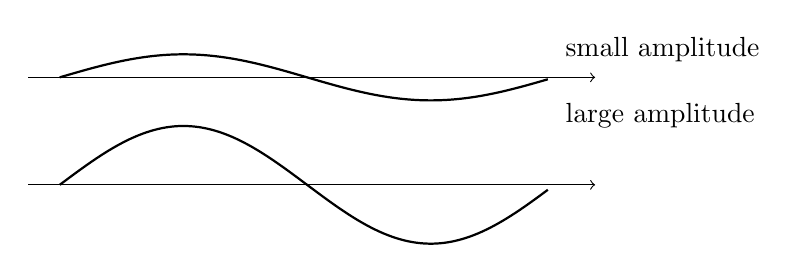
\begin{tikzpicture}[x=1cm,y=0.65cm]
\draw[->] (-0.4,0) -- (6.8,0);
\draw[->] (-0.4,-2.1) -- (6.8,-2.1);
\draw[thick] plot[domain=0:6.2,samples=120] (\x,{0.45*sin(\x r)});
\draw[thick] plot[domain=0:6.2,samples=120] (\x,{-2.1+1.15*sin(\x r)});
\draw (6.3,0.55) node[right]{small amplitude};
\draw (6.3,-0.75) node[right]{large amplitude};
\end{tikzpicture}
\caption{Two waves with the same frequency and wavelength but different amplitudes.}
\end{figure}

Quantum mechanically, if the wave contains \(n\) photons of one frequency \(\omega\), then its energy is also
\begin{equation}
E_{\text{wave}} = n\hbar\omega.
\end{equation}
Combining the two statements, we get the lecture's order-of-magnitude rule:
\begin{equation}
A^2 \propto n\hbar\omega.
\end{equation}
In particular, at fixed frequency,
\begin{equation}
A \propto \sqrt{n}.
\end{equation}

This must be kept in the cautious form used in the lecture. The exact normalization is not worked out here. One also has to understand the proportionality as referring to a fixed region of the wave, for example one wavelength, because otherwise the total energy can be made arbitrarily large simply by taking a longer stretch of wave. The audience explicitly raises this point, and the answer is that the lecture is indeed speaking only proportionally, not claiming an exact global formula.

There is another subtlety. In quantum mechanics the question is not perfectly sharp, because amplitude and phase are not simultaneously exact observables. So for one photon one should not speak as though there were a precisely defined classical amplitude attached to it. The safest lecture-faithful statement is the weaker one: for \(n=1\), the same formula gives the order of magnitude.

The lecture also pauses to clear up a common visual confusion. In the usual sketch of an electromagnetic wave moving along the \(x\)-axis, the vertical direction in the sine-wave drawing is not another spatial direction in which the photon wanders. It is the value of the electric or magnetic field. Only one axis in that picture is the direction of propagation.

\section{Which Relations Are General, and Which Are Special to Light?}

Having used the photon example, the lecture slows down and sorts the formulas on the board. This is an important beat in the argument. If we do not stop here, the later transition from photons to electrons will look like a jump instead of a controlled generalization.

\begin{figure}[t]
\centering

\includegraphics[width=0.82\textwidth]{lecture_02_figure_03.png}
\caption{Board layout separating wave definitions on the left from quantum and momentum formulas on the right.}
\end{figure}

The board itself makes the point visible. On the left sit the definitional wave quantities: \(f\), \(\omega\), and \(\lambda\). On the right sit the quantum and momentum relations. But not everything on the board has the same scope.

The definitions remain definitions. The relation
\begin{equation}
\omega=2\pi f
\end{equation}
is always true because it only translates one frequency unit into another. Likewise \(\lambda\) is just the wavelength by definition.

But the relations containing an explicit \(c\) are being fenced off. The equation \(\lambda f=c\) is special to waves moving at the speed of light. The momentum formula \(|p|=E/c\) is likewise special to radiation moving at the speed of light. On the other hand, the quantum relation \(E=\hbar\omega\) is much more general, and the lecture insists that the really lasting momentum statement is
\begin{equation}
p=\frac{h}{\lambda}.
\end{equation}

\begin{figure}[t]
\centering

\includegraphics[width=0.74\textwidth]{lecture_02_figure_04.png}
\caption{The moment at which the photon result is rewritten as the more general wavelength formula.}
\end{figure}

This is exactly why the lecture lingers over the formula
\begin{equation}
p_{\text{photon}}=\frac{hf}{c}=\frac{h}{\lambda}.
\end{equation}
The first expression still remembers that we are talking about a photon. The last one is the broader de Broglie relation. The same momentum-wavelength connection will be carried forward to slowly moving matter, whereas the explicit factor of \(c\) will not.

The lecture also remarks that \(\vec p=m\vec v\) is itself only a slow-particle approximation. There is an interpolation between that formula and the lightlike one, but it is not part of tonight's story. Tonight the contrast is between the nonrelativistic regime and the wave moving at the speed of light.

\section{Slow Matter Waves: Frequency, Wavelength, and Velocity}

Once \(p=h/\lambda\) has been promoted to a general statement, the next question is unavoidable. If an electron is also described by a wave, and if its wavelength is still tied to momentum by \(p=h/\lambda\), then what replaces \(\lambda f=c\) for a slowly moving electron, nucleus, or even a bowling ball?

Let us write the electron wave as \(\psi\). For a slowly moving particle, the needed extra fact is not a new wave formula but the nonrelativistic relation between energy and momentum:
\begin{equation}
E=\frac{1}{2}mv^2=\frac{p^2}{2m}.
\end{equation}
Now combine this with the wave-particle relations
\begin{equation}
E=hf,
\qquad
p=\frac{h}{\lambda}.
\end{equation}
Then
\begin{align}
hf &= \frac{p^2}{2m}
   = \frac{1}{2m}\left(\frac{h}{\lambda}\right)^2,
\end{align}
so after dividing by \(h\),
\begin{equation}
f=\frac{h}{2m\lambda^2}.
\end{equation}

\begin{figure}[t]
\centering

\includegraphics[width=0.64\textwidth]{lecture_02_figure_05.png}
\caption{Board layout for the nonrelativistic energy formula and the resulting matter-wave frequency relation.}
\end{figure}

This is the new frequency-wavelength relation for a slowly moving particle. It is strikingly different from the light-wave formula. For light,
\[
f\propto \frac{1}{\lambda}.
\]
For a nonrelativistic matter wave,
\[
f\propto \frac{1}{\lambda^2}.
\]
The lecture explicitly warns us not to memorize the result in isolation. Its importance is that it can always be rederived from two ingredients: the appropriate energy-momentum relation and the general de Broglie relation \(p=h/\lambda\).

\subsection{Question \& Answer}
\paragraph{Which velocity of a matter wave packet should be identified with the particle?}
Now the lecture pauses again, because a natural but misleading question arises. If we know \(f\) and \(\lambda\), can we not simply multiply them and get the velocity? We can, but not the velocity of the particle itself.

For one monochromatic component, the phase velocity is
\begin{equation}
v_{\phi}=f\lambda=\frac{h}{2m\lambda}.
\end{equation}
Because this depends on \(\lambda\), different wavelength components travel with different phase velocities. That is the hallmark of a dispersive medium.

\begin{figure}[t]
\centering
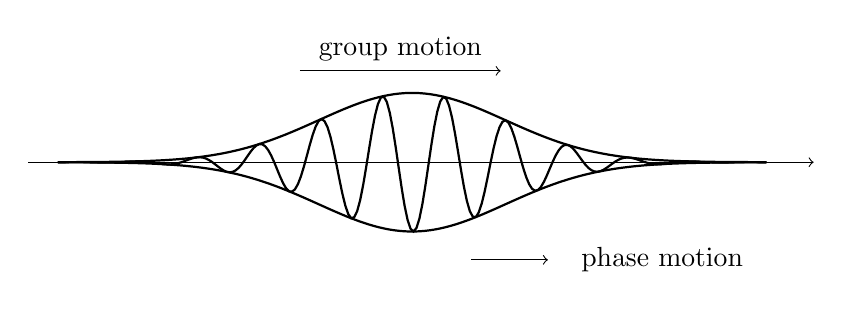
\begin{tikzpicture}[x=0.75cm,y=0.8cm]
\draw[->] (-0.5,0) -- (12.8,0);
\draw[thick] plot[domain=0:12,samples=140] (\x,{1.10*exp(-0.20*(\x-6)^2)});
\draw[thick] plot[domain=0:12,samples=140] (\x,{-1.10*exp(-0.20*(\x-6)^2)});
\draw[thick] plot[domain=0:12,samples=240] (\x,{1.10*exp(-0.20*(\x-6)^2)*sin(6*\x r)});
\draw[->] (4.1,1.45) -- (7.5,1.45);
\draw (5.8,1.8) node{group motion};
\draw[->] (7.0,-1.55) -- (8.3,-1.55);
\draw (8.7,-1.55) node[right]{phase motion};
\end{tikzpicture}
\caption{A schematic wave packet: the envelope and the interior crests generally move at different velocities.}
\end{figure}

The lecture therefore distinguishes two velocities. The phase velocity is the motion of the internal crests and troughs. The group velocity is the motion of the packet as a whole. It is the group velocity that we identify with the particle.

This is also the moment at which the lecture remarks that the result is really the Schr\"odinger equation in compressed form. Frequency encodes the time dependence of the wave; wavelength encodes its spatial dependence. An equation relating the two is already most of what the free Schr\"odinger equation does.

There is one important special case. If every wavelength moves with the same speed, then the crests and the packet move together. That is what happens for light in vacuum. There phase and group velocity coincide. For the nonrelativistic matter-wave relation above, they do not. The lecture even notes that the phase velocity may exceed the speed of light, but that carries no information; the physically relevant signal velocity is the group velocity.

\section{Finite Space, Periodic Space, and Quantized Momentum}

The lecture now changes scale and motivation. Up to this point we have been talking as though space were infinite, but the next step insists on a standard piece of good practice: first make the system finite, then understand the limit. Susskind's practical slogan is memorable and exact in spirit. Computers do not like infinity.

So let us reduce the problem to one dimension. There is a tempting first way to make space finite: take a segment of length \(L\), fix the ends, and let the wave bounce back and forth like a violin string. This is perfectly respectable physics, but it comes with a drawback. A wave moving to the right carries momentum to the right. When it reflects, the momentum flips sign. So the boundary has destroyed momentum conservation.

\subsection{Question \& Answer}
\paragraph{How do we make space finite without destroying momentum conservation?}
The lecture's answer is to identify the two ends. One may picture this as a circle if one likes, but only schematically. The important point is not ordinary geometry; it is periodicity. When the wave reaches one end, it reappears at the other and continues in the same direction. The endpoint is no longer special.

\begin{figure}[t]
\centering

\includegraphics[width=0.72\textwidth]{lecture_02_figure_06.png}
\caption{The board sketch with total length \(L\), presented as a schematic path rather than a literal geometric circle.}
\end{figure}

\begin{figure}[t]
\centering
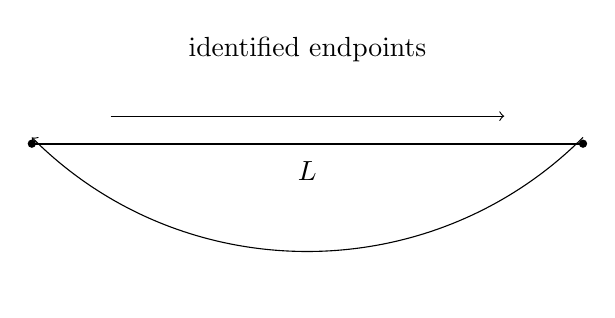
\begin{tikzpicture}[x=1cm,y=1cm]
\draw[thick] (0,0) -- (7,0);
\fill (0,0) circle (1.5pt);
\fill (7,0) circle (1.5pt);
\draw[->] (1.0,0.35) -- (6.0,0.35);
\draw (3.5,-0.35) node{\(L\)};
\draw[->,bend left=45] (7,0.08) to (0,0.08);
\draw (3.5,1.2) node{identified endpoints};
\end{tikzpicture}
\caption{A cleaned reconstruction of the periodic identification. The picture is schematic; the point is periodicity, not an embedded circle in two-dimensional space.}
\end{figure}

Once space is periodic, the allowed wavelengths are discrete. An integer number of wavelengths must fit around the total length:
\begin{equation}
\lambda_N=\frac{L}{N},
\qquad
N=1,2,3,\dots
\end{equation}
and therefore the allowed momenta are also discrete:
\begin{equation}
p_N=\frac{h}{\lambda_N}=\frac{Nh}{L}.
\end{equation}
This is the lecture's first clean example of momentum quantization.

If \(L\) is very large, the spacing \(h/L\) between allowed momenta is very small, so the spectrum looks almost continuous. If \(L\) is made smaller, the spacing grows. But the main point is structural: momentum comes in discrete multiples because only certain wavelengths are compatible with periodicity.

The audience then asks about a packetized wave, and the answer is equally important. A wave packet is a superposition of plane waves. In periodic space, that means a superposition of the allowed discrete modes. This is simply Fourier analysis with a discrete momentum basis.

The lecture also recasts the same fact for a genuine circular wire of radius \(r\), with circumference \(L=2\pi r\). To avoid the notational stumble that occurs on the board, let us keep \(N\) for the mode label and \(J\) for angular momentum. Then
\begin{equation}
p_N=\frac{Nh}{2\pi r},
\qquad
J = rp_N = N\hbar.
\end{equation}
So angular momentum is quantized in units of \(\hbar\), while the momentum spacing itself depends on the size of the circle.

\section{Quantum Mechanics, the Harmonic Oscillator, and the First Picture of a Field}

After the break the lecture says, in effect, that we now have to enter the real world of quantum mechanics a little bit. The first object introduced is the commutator:
\begin{equation}
[A,B]=AB-BA.
\end{equation}
Its reverse-order version differs by a sign,
\begin{equation}
[B,A]=-[A,B].
\end{equation}
Here the commutator is an algebraic operation, not a temporal instruction to measure one thing and then another. The lecture uses it as the test for simultaneous measurability: if two observables commute, they can be measured together; if they do not, the attempt to measure one interferes with the other.

For an ordinary nonrelativistic particle, the position components commute with one another, and the momentum components commute with one another:
\begin{equation}
[x,y]=[y,z]=[z,x]=0,
\qquad
[p_x,p_y]=[p_y,p_z]=[p_z,p_x]=0.
\end{equation}
But the corresponding position and momentum components do not:
\begin{equation}
[x,p_x]=[y,p_y]=[z,p_z]=i\hbar.
\end{equation}
Mixed components such as \(x\) and \(p_y\) do commute. The lecture briefly notes that this simple position-momentum discussion applies most cleanly to nonrelativistic particles; for photons the notion of position is subtler, and that subtlety is postponed.

The real destination is the harmonic oscillator. It appears here because waves oscillate. A field mode of definite frequency is already halfway to an oscillator. The quantum-mechanical novelty is that the oscillator does not carry arbitrary energy. Its energy levels are discrete. In the lecture the zero of energy is shifted so that the lowest level sits at \(0\), not at \(\frac12\hbar\omega\). With that convention,
\begin{equation}
E_n = n\hbar\omega,
\qquad
n=0,1,2,\dots
\end{equation}
and the state with energy \(E_n\) is denoted by the ket \(|n\rangle\).

\begin{figure}[t]
\centering
\begin{tikzpicture}[x=1cm,y=0.9cm]
\draw[->] (0,0) -- (0,5.35);
\draw (0,5.5) node[above]{energy};
\foreach \y/\lab in {0.6/{0},1.6/{\hbar\omega},2.6/{2\hbar\omega},3.6/{3\hbar\omega},4.6/{n\hbar\omega}}
{
  \draw[thick] (0.2,\y) -- (2.2,\y);
  \draw (-0.25,\y) node[left]{\(\lab\)};
}
\draw[->,thick] (2.8,0.68) -- (2.8,1.52);
\draw (3.2,1.1) node[right]{\(a_+\)};
\draw[->,thick] (3.7,1.52) -- (3.7,0.68);
\draw (4.1,1.1) node[right]{\(a_-\)};
\end{tikzpicture}
\caption{A cleaned energy-level picture of the shifted harmonic oscillator used in the lecture.}
\end{figure}

Now come the raising and lowering operators, written on the board as \(A+\) and \(A-\), and here written as \(a_+\) and \(a_-\):
\begin{align}
a_+|n\rangle &= \sqrt{n+1}\,|n+1\rangle,\\
a_-|n\rangle &= \sqrt{n}\,|n-1\rangle,\\
a_-|0\rangle &= 0.
\end{align}
These operators move us one step up or down the ladder of states, thereby adding or removing one quantum of energy of frequency \(\omega\).

Their algebra is already revealing. Acting in one order gives
\begin{equation}
a_+a_-|n\rangle = n|n\rangle,
\end{equation}
while the reverse order gives
\begin{equation}
a_-a_+|n\rangle = (n+1)|n\rangle.
\end{equation}
So the two orders do not agree. Applied to every state, this implies
\begin{equation}
[a_-,a_+]=1.
\end{equation}
In the shifted convention being used here, the Hamiltonian may be written as
\begin{equation}
H=\hbar\omega\,a_+a_-.
\end{equation}

What do these operators mean physically? The lecture is careful here. One does not ordinarily measure \(a_+\) and \(a_-\) separately as direct observables. Their noncommutativity reflects the fact that they encode amplitude-and-phase information that cannot be made simultaneously sharp. But mathematically they do something definite: they create and annihilate quanta. If the oscillator is an electromagnetic mode, the quanta are photons.

Now the lecture returns to the periodic world of length \(L\). Each allowed wavelength \(\lambda_N=L/N\) carries an allowed frequency \(\omega_N\). Each such mode is one harmonic oscillator. A field is therefore a whole collection of oscillators, one for each allowed mode. The state of the field is not labeled by one integer but by an infinite list:
\begin{equation}
|n_1,n_2,n_3,\dots\rangle.
\end{equation}
Here the notation has to be kept clean. The mode label is \(N\). The occupation number of a given mode is \(n_N\). The audience notices the danger of confusing those two integers, and the lecture explicitly pauses to separate them.

The violin-string analogy is the right one. There is a fundamental mode, then higher harmonics, then higher still. Each mode has its own frequency, and each mode can carry zero, one, two, or more quanta. The total energy of the field is then built mode by mode:
\begin{equation}
E=\sum_{N} n_N \hbar\omega_N.
\end{equation}
A quantum field, in this first elementary picture, is exactly this: a collection of harmonic oscillators together with creation and annihilation operators for each oscillator.

That is why the lecture ends by tying the whole discussion back to particle physics experiments. Particles with given energy and momentum come in. Particles with other energies and momenta go out. Mathematically, we remove quanta from an initial state and add quanta to a final state. Creation and annihilation operators are the symbols that do that work. They are the language in which particle processes are written.

\section{Summary}

The lecture opens by delaying the definition of quantum field theory and instead assembling the mathematics of oscillation that the subject keeps using. From exponentials, sines, and cosines we move to frequency and wavelength, from there to the one-quantum energy \(E=\hbar\omega\), and then to the photon momentum formula \(p=h/\lambda\). After the audience's question about amplitude, the lecture sorts the formulas by generality and then turns the same wave-particle dictionary onto slowly moving matter, where the relation \(f\propto 1/\lambda^2\) leads naturally to the distinction between phase velocity and group velocity. Periodic space then makes momentum discrete without sacrificing momentum conservation. After the break, the harmonic oscillator provides the missing quantum-mechanical machinery, and the promised picture finally appears: a quantum field is a collection of oscillators, one for each allowed mode, together with operators that add and remove quanta in those modes.